\section{Excluding an isolated compact piece}
\label{sec:compact-piece}

We now work with a global absolute minimizer of $E_0$ whose complement is
connected. The target is to exclude a separated compact piece of positive
length that contains a regular arc. The main idea is to split the gradient into the
field produced by that compact part and a field harmonic across it. Translating
the compact part preserves its length and its own Dirichlet energy. The remaining
interaction is harmonic in the translation parameter, so minimality forces it
to be constant. We then vary the jump across one regular arc to show that the
entire gradient vanishes, making the compact part removable.

The strategic electrostatic analogy is Earnshaw's no-stable-equilibrium
principle; see Rahi, Kardar, and Emig \cite[pp.~1--2]{rahi_kardar_emig2009}
for a modern discussion.  This analogy motivates the translation strategy,
but does not provide a sign rule for bounded-domain Dirichlet variations.
The whole-plane projection, cutoff, finite-translation, and jump-variation
arguments needed here are supplied below.

Compact translations and independently variable jumps on regular arcs also
enter Deangelis's proof of global classification \cite{deangelis2026}.
His argument uses relaxed second variations, equality in a planar Hodge
identity, and holomorphic rigidity. The finite translations below produce
a scalar harmonic interaction, whose constancy can be tested against every
compactly supported change of the jump.

Throughout this section, $B_R=B_R(0)\subset\mathbb R^2$. A function on the
complement of a set of zero area, and its gradient density, are assigned arbitrary
values on that set when integrated with respect to area. For a scalar function
defined off a closed set, compact support means compact essential support
in the ambient plane; the support is allowed to meet that closed set.
For a scalar function
or vector field $a$, its translate by $t\in\mathbb R^2$ is
\[
 a_t(x)=a(x-t).
\]
For a set $A$, write $A_t=A+t=\{x+t:x\in A\}$.
We use the distributional conventions
\[
 \operatorname{curl}(a_1,a_2)=\partial_1a_2-\partial_2a_1,
 \qquad \nabla^\perp b=(-\partial_2b,\partial_1b).
\]
Thus $\Delta a=\nabla\operatorname{div}a+
\nabla^\perp\operatorname{curl}a$.

\begin{proposition}[Exclusion of a separated compact piece]
\label{prop:compact-piece}
Let $H\subset\mathbb R^2$ be closed, rectifiable, and locally of finite
$\mathcal H^1$ measure, and assume $D=\mathbb R^2\setminus H$ is connected.
Let $(v,H)$ be an absolute minimizer of $E_0$ under compactly supported
comparisons, with
\[
 v\in W^{1,2}(B_R\setminus H)\quad(R>0),\qquad
 \int_{B_R}|\nabla v|^2\leq C(1+R)\quad(R\geq1).
\]
There is no compact set $A\subset H$ satisfying all of the following:
\begin{enumerate}
 \item $\mathcal H^1(A)>0$;
 \item $B=H\setminus A$ is closed and $\operatorname{dist}(A,B)>0$,
       with the distance interpreted as $+\infty$ if $B=\varnothing$;
 \item $A$ contains an open subarc of $H$ that is an embedded $C^1$ arc.
\end{enumerate}
In the third condition, an open subarc means that some open neighborhood
meets $H$ in just that arc.
\end{proposition}

Here is the decomposition that organizes the argument. Suppose provisionally
that $H=A\cup B$, where $A$ is compact and separated from the closed remainder
$B$. Choose a smooth cutoff $\chi$ supported away from $B$ and equal to one
near $A$, so that $h=\chi v$ carries the part of the function near $A$.
The projection in Lemma~\ref{lem:compact-projection} constructs a potential
$\phi$ whose gradient is square integrable on the whole plane. We then set
\[
 F=\chi v-\phi,\qquad f=(1-\chi)v+\phi,\qquad v=f+F.
\]
The proof of Proposition~\ref{prop:compact-piece} will show that $f$ is
harmonic across $A$, while $F$ has its only possible jump on $A$ and decays
at infinity. Thus $f$ can be held fixed while $F$ and the compact set are
translated together. The three lemmas below construct this split, justify
the finite-disk comparisons, and identify the resulting harmonic
interaction. The proposition then uses independent changes of the jump to
force both gradient contributions to vanish.

\subsection{A finite-energy field carrying the compact jump}

The first lemma constructs a finite-energy field whose only possible jump
lies on a prescribed compact set. The decay at infinity will allow us to
translate this field and then return to the original function far away.

\begin{lemma}[Projection of a compactly supported function]
\label{lem:compact-projection}
Let $A\subset\mathbb R^2$ be compact and have zero area. Suppose
$h\in W^{1,2}(\mathbb R^2\setminus A)$ has compact support, and write
$e=\nabla h$ for its gradient density. Let
\[
 Z=\overline{\{\nabla\zeta:\zeta\in C_c^\infty(\mathbb R^2)\}}
       ^{\,L^2(\mathbb R^2;\mathbb R^2)},
\]
and let $Q$ be the orthogonal projection onto $Z$. There is a unique
$\phi\in W^{1,2}_{\mathrm{loc}}(\mathbb R^2)$ satisfying
$\nabla\phi=Qe$ and tending to zero at infinity. Set
\[
 F=h-\phi\quad\hbox{on }\mathbb R^2\setminus A,
 \qquad p=e-\nabla\phi\quad\hbox{on }\mathbb R^2.
\]
Then $p\in L^2(\mathbb R^2;\mathbb R^2)$,
$F\in W^{1,2}(B_R\setminus A)$ for every $R>0$,
and $\nabla F=p$ off $A$. Distributionally on the whole plane,
\begin{equation}
 \operatorname{div}p=0,\qquad
 \operatorname{supp}(\operatorname{curl}p)\subset A,\qquad
 \Delta p=\nabla^\perp\operatorname{curl}p.
 \label{eq:compact-field-equations}
\end{equation}
Outside a sufficiently large disk, $F$ and $p$ are smooth, and
\begin{equation}
 F(x)=O(|x|^{-1}),\qquad
 |\nabla^k F(x)|=O_k(|x|^{-1-k})\quad(k\geq1).
 \label{eq:compact-field-decay}
\end{equation}
In particular $p(x)=O(|x|^{-2})$ there.
\end{lemma}

\begin{proof}
Every element of $Z$ is the gradient of a scalar function in
$W^{1,2}_{\mathrm{loc}}(\mathbb R^2)$. Indeed, for a defining sequence
of gradients, subtract the mean of each potential on $B_1$. Poincar\'e's
inequality, first on $B_1$ and then on larger overlapping balls, makes these
potentials Cauchy in $W^{1,2}$ on every fixed ball. Apply this to $Qe$.

The projection identity gives
\[
 \int_{\mathbb R^2}(e-\nabla\phi)\cdot\nabla\zeta=0
       \qquad(\zeta\in C_c^\infty(\mathbb R^2)).
\]
Consequently $\Delta\phi=\operatorname{div}e$ and
$\operatorname{div}p=0$. Since $e$ has compact support, $\phi$ is harmonic
outside a disk. Its gradient has finite energy on the whole plane.
The Fourier expansion of a single-valued harmonic function on the exterior
of a disk consists of a constant, a logarithmic term, and modes $r^{\pm n}$
for integers $n\geq1$. Finite Dirichlet energy excludes the logarithmic and
growing modes. Subtracting the remaining constant gives
\[
 \phi(x)=O(|x|^{-1}),\qquad
 |\nabla^k\phi(x)|=O_k(|x|^{-1-k})\quad(k\geq1).
\]
This normalization is unique. The bounds follow, for example, by estimating
the decaying Fourier series outside a larger concentric disk.

Off $A$, the field $p$ is the weak gradient of $h-\phi$, so its curl
vanishes there. This proves the support assertion in
\eqref{eq:compact-field-equations}; the last identity follows from
$\operatorname{div}p=0$. Finally $h=0$ outside a disk, so $F=-\phi$ there.
\end{proof}

\subsection{The energy comparison and its harmonic interaction}

The comparison translates $F$ together with $A$ and also changes its jump
by an independent field $P$ with amplitude $\sigma$. We include the distant
cutoff that makes this an admissible compact comparison; all interaction
integrals below converge absolutely.

\begin{lemma}[Translated comparison]
\label{lem:translated-comparison}
Let $H=A\cup B\subset\mathbb R^2$ be closed, rectifiable, and locally of finite
$\mathcal H^1$ measure, where $A$ is compact, $B$ is closed, and
$\operatorname{dist}(A,B)>0$. Let $(v,H)$ be an absolute minimizer of
$E_0$ under compactly supported comparisons, with
\[
 v\in W^{1,2}(B_R\setminus H)\quad(R>0),\qquad
 \int_{B_R}|\nabla v|^2\leq C(1+R)\quad(R\geq1).
\]
Suppose $v=f+F$ off $H$, where
$f\in W^{1,2}(B_R\setminus B)$ for every $R>0$, and
$(F,p)$ is obtained from a compactly supported
$h\in W^{1,2}(\mathbb R^2\setminus A)$ by
Lemma~\ref{lem:compact-projection}. Put $G=\nabla v-p$, and assume
\[
 G=\nabla f\text{ off }B,\qquad
 \int_{B_R}|G|^2\leq C'(1+R)\quad(R\geq1).
\]
For any compactly supported
$h'\in W^{1,2}(\mathbb R^2\setminus A)$, let $(P,q)$ be its counterpart
of $(F,p)$ in Lemma~\ref{lem:compact-projection}. Choose $\delta>0$ so
that $A_t\cap B=\varnothing$ whenever $|t|<\delta$. Define
\[
 I_p(t)=\int_{\mathbb R^2}G\cdot p_t,
 \qquad I_q(t)=\int_{\mathbb R^2}G\cdot q_t.
\]
Then these integrals converge absolutely, and for every $|t|<\delta$
and $\sigma\in\mathbb R$,
\begin{equation}
 0\leq 2\bigl(I_p(t)-I_p(0)\bigr)
     +2\sigma\bigl(I_q(t)+\langle p,q\rangle_{L^2}\bigr)
     +\sigma^2\|q\|_{L^2}^2.
 \label{eq:translated-energy}
\end{equation}
\end{lemma}

\begin{proof}
Fix $t$ and $\sigma$. For large $R$, let $\eta_R$ be smooth, equal to
one near $\overline B_R$, zero near $\mathbb R^2\setminus B_{2R}$,
and satisfy $|\nabla\eta_R|\leq C/R$. Use the set
$J=B\cup A_t$ and the function
\[
 V_R=\begin{cases}
 f+F_t+\sigma P_t,&x\in B_R\setminus J,\\
 v+\eta_R(F_t-F+\sigma P_t),&x\in(B_{2R}\setminus\overline B_R)\setminus J,\\
 v,&x\notin B_{2R}\cup J.
 \end{cases}
\]
Take $R$ large enough to contain the compact pieces and all supports used
in the projection constructions. The first formula is Sobolev off $J$,
since $f$ extends across $A$ and $F_t,P_t$ are Sobolev off $A_t$.
The formulas agree near the interfaces because $v=f+F$ off $H$.
The set $J$ is rectifiable because $A$ and $B$ are subsets of the
rectifiable set $H$, and translation preserves rectifiability.
Thus $(V_R,J)$ is admissible. Its change from $(v,H)$ has compact support
in a bounded open disk slightly larger than $B_{2R}$.
In that disk the length terms cancel exactly, since $A_t$ is disjoint
from $B$ and $\mathcal H^1(A_t)=\mathcal H^1(A)$.

On the gluing annulus, the exterior estimates of
Lemma~\ref{lem:compact-projection} give
\[
 \bigl\|\nabla\bigl[\eta_R(F_t-F+\sigma P_t)\bigr]\bigr\|_{L^2}
       \leq C_{t,h,h'}(1+|\sigma|)R^{-1}.
\]
The change of Dirichlet energy on that annulus is therefore
$O((1+|\sigma|)R^{-1/2})+O((1+|\sigma|)^2R^{-2})$, which tends to zero.
Here we used $\|\nabla v\|_{L^2(B_{2R})}=O(R^{1/2})$.

For completeness, the interactions are absolutely integrable at infinity:
on a dyadic annulus of radius $s$,
\[
 \|G\|_{L^2}=O(s^{1/2}),\qquad
 \|p_t\|_{L^2}+\|q_t\|_{L^2}=O(s^{-1}),
\]
so their products have integrals $O(s^{-1/2})$, summable over dyadic
annuli. On bounded sets the products are integrable by Cauchy--Schwarz.

Inside $B_R$, the two gradients are $G+p_t+\sigma q_t$ and $G+p$.
Expand their squared norms in the finite comparison, then let
$R\to\infty$. Translation invariance gives
\[
 \|p_t\|_2=\|p\|_2,\quad \|q_t\|_2=\|q\|_2,\quad
 \langle p_t,q_t\rangle=\langle p,q\rangle.
\]
These equalities and the preceding estimates yield
\eqref{eq:translated-energy}. In particular, no subtraction of infinite
whole-plane Dirichlet energies is involved.
\end{proof}

\begin{lemma}[Harmonicity and constancy of the interaction]
\label{lem:harmonic-interaction}
In the setting of Lemma~\ref{lem:translated-comparison}, suppose in addition
that $f$ is harmonic on $O=\mathbb R^2\setminus B$.
After decreasing $\delta$ if necessary, $I_p$ is harmonic on
$B_\delta(0)$ as a function of the translation parameter. Consequently
\begin{equation}
 I_p(t)=I_p(0),\qquad
 I_q(t)=-\langle p,q\rangle_{L^2}
       \quad(|t|<\delta)
 \label{eq:constant-interactions}
\end{equation}
for every compactly supported $h'$ allowed in
Lemma~\ref{lem:translated-comparison}.
\end{lemma}

\begin{proof}
Choose $\zeta\in C_c^\infty(O)$ equal to one on a neighborhood of all
$A_t$ for $|t|<\delta$, and split $I_p$ using $\zeta G$ and
$(1-\zeta)G$. The field $\zeta G$ is a smooth compactly supported
test field on the whole plane, because $G=\nabla f$ on $O$.
Distributional differentiation and
\eqref{eq:compact-field-equations} give
\[
 \Delta_t\langle p_t,\zeta G\rangle
   =\langle\nabla^\perp\operatorname{curl}p_t,\zeta G\rangle
   =-\langle\operatorname{curl}p_t,\operatorname{curl}(\zeta G)\rangle=0.
\]
Indeed $\operatorname{curl}p_t$ is supported on $A_t$, and
$\operatorname{curl}(\zeta G)=0$ on a neighborhood of $A_t$.

On the support of $1-\zeta$, the field $p_t$ is harmonic and smooth,
uniformly separated from $A_t$ on bounded sets. At infinity, its
$k$th translation derivatives are $O(|x|^{-2-k})$. Together with the
growth bound for $G$, the dyadic estimate in the preceding proof gives
an integrable bound for each differentiated integrand, locally uniformly
in $t$. Differentiation under the second integral is therefore justified,
and its translation Laplacian also vanishes. Thus $I_p$ is harmonic.

Taking $\sigma=0$ in \eqref{eq:translated-energy} shows that $I_p$
has a minimum at the origin. The minimum principle makes it constant
on the translation disk. For any fixed $t$, the remaining right side
of \eqref{eq:translated-energy} is a quadratic polynomial in $\sigma$
with zero constant term, nonnegative for all real $\sigma$. Its linear
coefficient must vanish. This proves \eqref{eq:constant-interactions}.
\end{proof}

\subsection{Jump variations force the whole field to vanish}

The preceding lemmas turn the energy inequality into an equality for
every compactly supported value variation. We now use variations whose
two traces on a regular arc differ. Their arbitrary jumps measure the
normal derivative of the harmonic function $f$ on every nearby translate
of the arc.



\begin{proof}[Proof of Proposition~\ref{prop:compact-piece}]
Suppose such an $A$ exists, and put $O=\mathbb R^2\setminus B$.
Because $H$ has zero area, $D$ is dense in the plane. The set $O$
contains the connected set $D$ and is contained in its closure, so
$O$ is connected.

Set $m=\nabla v$ off $H$. Comparing $v$ with $v+s\psi$ for
$\psi\in C_c^\infty(\mathbb R^2)$ and both signs of $s$ gives
\begin{equation}
 \operatorname{div}m=0\quad\hbox{in }\mathcal D'(\mathbb R^2).
 \label{eq:whole-plane-divergence}
\end{equation}
Choose $\chi\in C_c^\infty(O)$ equal to one on a neighborhood of $A$.
The function $h=\chi v$, extended by zero near $B$, belongs to
$W^{1,2}(\mathbb R^2\setminus A)$ and has compact support.
Apply Lemma~\ref{lem:compact-projection}, obtaining $\phi,F,p$, and define
\[
 f=(1-\chi)v+\phi\quad\hbox{on }O,\qquad G=m-p.
\]
Near $A$, the first term in $f$ vanishes; thus $f$ extends across $A$
and belongs to $W^{1,2}(B_R\setminus B)$ for every $R$.
Off $H$ we have $v=f+F$ and $G=\nabla f$. These identities hold
almost everywhere on $O$, since $A$ has zero area.
By \eqref{eq:whole-plane-divergence} and
\eqref{eq:compact-field-equations}, $\operatorname{div}G=0$ on the
whole plane. It follows that $f$ is harmonic on $O$. Also
\begin{equation}
 \int_{B_R}|G|^2
      \leq 2\int_{B_R}|m|^2+2\|p\|_2^2
      \leq C_1(1+R)\qquad(R\geq1).
 \label{eq:external-field-growth}
\end{equation}
We have separated $v$ into a function $f$ harmonic through $A$ and a
function $F$ whose possible jumps lie on $A$. Figure~\ref{fig:compact-translation}
shows how the comparison keeps $B$ and $f$ fixed while translating $A$,
$F$, and an independent jump variation $P$ together. A distant cutoff
returns the comparison to the original function.
\begin{figure}[tbp]
  \centering
  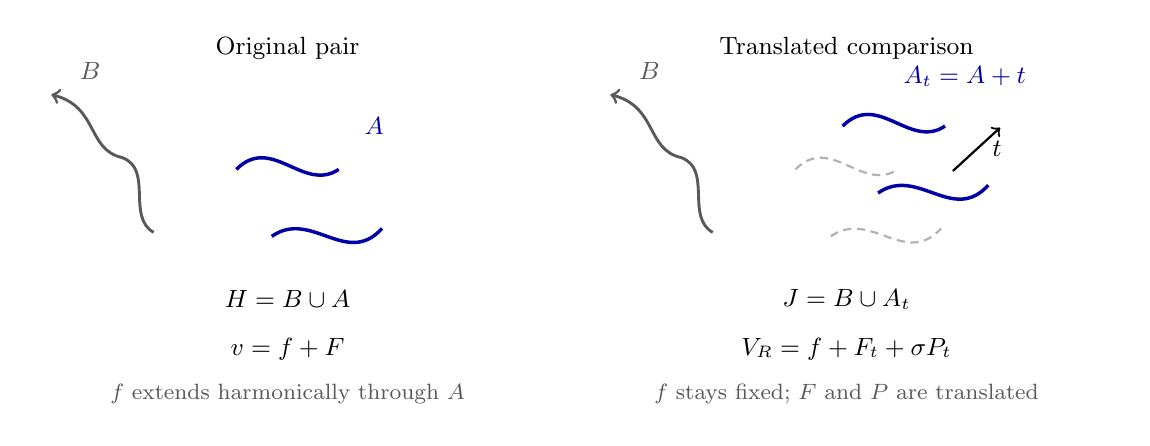
\begin{tikzpicture}[x=1cm,y=1cm,
      every node/.style={font=\small},
      fixed/.style={draw=black!65,line width=1.05pt},
      moving/.style={draw=blue!65!black,line width=1.25pt},
      old/.style={draw=black!30,line width=.8pt,densely dashed}]
    \path[use as bounding box] (-.05,-1.35) rectangle (13.85,3.6);

    \begin{scope}
      \node[anchor=north] at (3.25,3.6) {Original pair};
      \draw[fixed,<-] (.25,2.75)
        .. controls (.85,2.6) and (.7,2.05) .. (1.15,1.95)
        .. controls (1.55,1.8) and (1.2,1.2) .. (1.55,1.0);
      \node[anchor=east,text=black!65] at (1.0,3.05) {$B$};
      \draw[moving] (2.6,1.8)
        .. controls (3.05,2.25) and (3.45,1.5) .. (3.9,1.8);
      \draw[moving] (3.05,.95)
        .. controls (3.55,1.3) and (4.0,.55) .. (4.45,1.05);
      \node[text=blue!65!black] at (4.35,2.35) {$A$};
      \node at (3.25,.15) {$H=B\cup A$};
      \node at (3.25,-.48) {$v=f+F$};
      \node[font=\footnotesize,text=black!65] at (3.25,-1.05)
        {$f$ extends harmonically through $A$};
    \end{scope}

    \begin{scope}[xshift=7.1cm]
      \node[anchor=north] at (3.25,3.6) {Translated comparison};
      \draw[fixed,<-] (.25,2.75)
        .. controls (.85,2.6) and (.7,2.05) .. (1.15,1.95)
        .. controls (1.55,1.8) and (1.2,1.2) .. (1.55,1.0);
      \node[anchor=east,text=black!65] at (1.0,3.05) {$B$};
      \draw[old] (2.6,1.8)
        .. controls (3.05,2.25) and (3.45,1.5) .. (3.9,1.8);
      \draw[old] (3.05,.95)
        .. controls (3.55,1.3) and (4.0,.55) .. (4.45,1.05);
      \begin{scope}[shift={(.6,.55)}]
        \draw[moving] (2.6,1.8)
          .. controls (3.05,2.25) and (3.45,1.5) .. (3.9,1.8);
        \draw[moving] (3.05,.95)
          .. controls (3.55,1.3) and (4.0,.55) .. (4.45,1.05);
      \end{scope}
      \draw[->,line width=.8pt] (4.6,1.78) -- (5.2,2.33)
        node[midway,right=2pt] {$t$};
      \node[text=blue!65!black] at (4.75,2.98) {$A_t=A+t$};
      \node at (3.25,.15) {$J=B\cup A_t$};
      \node at (3.25,-.48) {$V_R=f+F_t+\sigma P_t$};
      \node[font=\footnotesize,text=black!65] at (3.25,-1.05)
        {$f$ stays fixed; $F$ and $P$ are translated};
    \end{scope}
  \end{tikzpicture}
  \caption{The comparison associated with a hypothetical separated compact
  piece $A$.  The remainder $B$ is fixed, while $A$ is translated by a small
  vector $t$ with $A_t\cap B=\varnothing$; the dashed curves mark its former
  position.  The displayed formula for $V_R$ holds in the inner comparison
  disk.  Far away, a cutoff returns the function to $v$.  The drawings are
  schematic: $A$ may contain several components, and no regularity of all of
  $A$ or $B$ is asserted.  The functions $F$ and $P$ need not have compact
  support.}
  \label{fig:compact-translation}
\end{figure}


All hypotheses of Lemmas~\ref{lem:translated-comparison}
and~\ref{lem:harmonic-interaction} now hold. In particular,
\eqref{eq:constant-interactions} holds for every compactly supported
$h'\in W^{1,2}(\mathbb R^2\setminus A)$.

We explain how to remove the projected potential from these interactions.
Let $\phi'$ be the normalized potential associated with such an $h'$.
Since $\operatorname{div}G=0$, testing with $\theta_R\phi'_t$, where
$\theta_R$ is a smooth cutoff on $B_{2R}$ equal to one on $B_R$, gives
\[
 \int\theta_R G\cdot\nabla\phi'_t
       =-\int G\cdot\nabla\theta_R\,\phi'_t.
\]
The compactly supported Sobolev test is justified by smooth approximation,
because $G\in L^2_{\mathrm{loc}}$. By the exterior normalization
$\phi'_t=O(R^{-1})$ on the cutoff annulus and
\eqref{eq:external-field-growth}, the right side is $O(R^{-1/2})$.
The uncut left integrand is absolutely integrable by the same dyadic
estimate used in Lemma~\ref{lem:translated-comparison}. Hence
\begin{equation}
 \int_{\mathbb R^2}G\cdot\nabla\phi'_t=0,
 \qquad
 I_q(t)=\int_{\mathbb R^2}G\cdot(\nabla h')_t.
 \label{eq:remove-projection}
\end{equation}
This step uses the distributional equation and decay, not a claim that
$G$ belongs to global $L^2$.

Take a smaller part of the regular arc in $A$. After a rigid change of
coordinates, it has the form
\[
 \gamma(s)=(s,\kappa(s)),\qquad s\in I,
\]
where $I$ is a bounded interval and $\kappa$ is $C^1$ on a neighborhood of
$\overline I$. Choose $I$ and $a>0$ so that the graph strip
$\{(s,\kappa(s)+r):s\in I,\ |r|<a\}$ is relatively compact in $O$
and meets $H$ only in the continuation of this arc. Let $n(s)$ be one
of its continuous unit normals. Choose
$\eta\in C_c^\infty((-a,a))$ with $\eta(0)=1$.
For every $\beta\in C_c^\infty(I)$ define, on the strip,
\[
 h'_\beta(x_1,x_2)
   =\mathbf 1_{\{x_2>\kappa(x_1)\}}\,
        \beta(x_1)\eta(x_2-\kappa(x_1)),
\]
and extend it by zero outside the strip. Its support avoids the ends
and the outer edge of the strip. Since $\kappa$ is $C^1$, this function is
Sobolev on each side, has its only jump on $A$, and belongs to
$W^{1,2}(\mathbb R^2\setminus A)$. Its trace difference on the arc
is $\beta$. Thus only $C^1$ regularity of the arc is needed. Denote by
$q_\beta$ the field associated with $h'_\beta$ by
Lemma~\ref{lem:compact-projection}.

Decrease the translation disk once so that every translate of this
fixed strip stays in $O$. Integration by parts on its translated upper
side, where $f$ is harmonic, and \eqref{eq:remove-projection} give
\begin{equation}
 I_{q_\beta}(t)
   =\pm\int_I\beta(s)\,
       n(s)\cdot\nabla f(\gamma(s)+t)\,|\gamma'(s)|\,ds.
 \label{eq:jump-flux}
\end{equation}
There are no other boundary terms, because the test vanishes near all
other edges. Translation preserves the normal $n(s)$.

By \eqref{eq:constant-interactions}, the left side of
\eqref{eq:jump-flux} is independent of $t$, for every $\beta$.
The fundamental lemma for tests on $I$ and continuity imply
\[
 n(s)\cdot\nabla f(\gamma(s)+t)
      =n(s)\cdot\nabla f(\gamma(s))
       \qquad(s\in I, |t|<\delta).
\]
Fix an interior $s_0$. A single fixed directional derivative of $f$
is constant on a disk about $\gamma(s_0)$. In two dimensions this
forces a harmonic function to be affine there: in rotated coordinates
$\partial_1 f=c$ gives $f=cx_1+a(x_2)$, and $\Delta f=0$ gives
$a''=0$. Unique continuation for harmonic functions makes $f$ affine
on the connected open set $O$.

Thus $G$ is a constant vector almost everywhere in the plane.
The growth estimate \eqref{eq:external-field-growth} forces that vector
to be zero. Now take $h'=h$, so $q=p$, in
\eqref{eq:constant-interactions}. It gives $\|p\|_2^2=0$.
Consequently $m=G+p=0$ almost everywhere on $D$. Since $D$ is connected,
$v$ is constant there. Extend this constant across $A$ and use the closed rectifiable set
$B$. This is an admissible comparison supported on the compact set $A$:
the function agrees with $v$ almost everywhere, the Dirichlet energy
is unchanged, and the length decreases by $\mathcal H^1(A)>0$.
This contradicts absolute minimality.
\end{proof}
